\chapter{Komponenttipankki}
Tässä osuudessa on kerätty yhteen tekstistä löytyvät komponenttilaatikot. 

\begin{tcolorbox}[title=Vastuksen arvo]
Jos sinulla ei ole käytössä yleismittaria oikean vastuksen arvon mittaamiseen, tai haluat harjoitella vastusten värikoodien lukemista, vastusten värikoodit löydät sivulta \pageref{varikoodit}.

Nyt tarvitaan $220\Omega$ vastus eli jompi kumpi alla olevista vaihtoehdoista:

\begin{center}
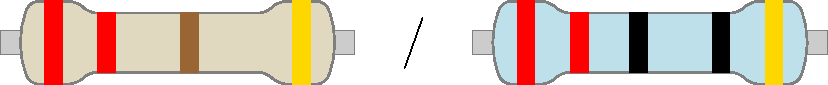
\includegraphics[width=0.5\textwidth]{kuvat/220.pdf}
\end{center}
\end{tcolorbox}

\begin{tcolorbox}[title=LEDin kytkeminen,colback=blue!10,colbacktitle=purple!90]\label{box:led}
Huomaa, että on merkitystä kummin päin LED kytketään koekytkentälevylle! 

LEDissä on kaksi jalkaa, joista toinen on pidempi. LEDin muovi on toiselta puolelta kaareva, ja toiselta siinä on suora leikkaus, lyhyempi jalka on suoran leikkauksen puolella. Lyhyemmän jalan nimi on katodi ja pidemmän jalan anodi.

\begin{minipage}{0.5\textwidth}
Piirrosmerkissä:
\begin{center}
\begin{tikzpicture}
%\node at (-1,0) {anodi};
\draw (0,0) node[left,text width=1.5cm] {anodi\\ pitkä jalka} to[led,o-o] (2,0) node[right,text width=2cm] {katodi\\lyhyt jalka};
\end{tikzpicture}
\end{center}
\end{minipage}
\begin{minipage}{0.5\textwidth}
\begin{tikzpicture}
\node (led) at (0,0) {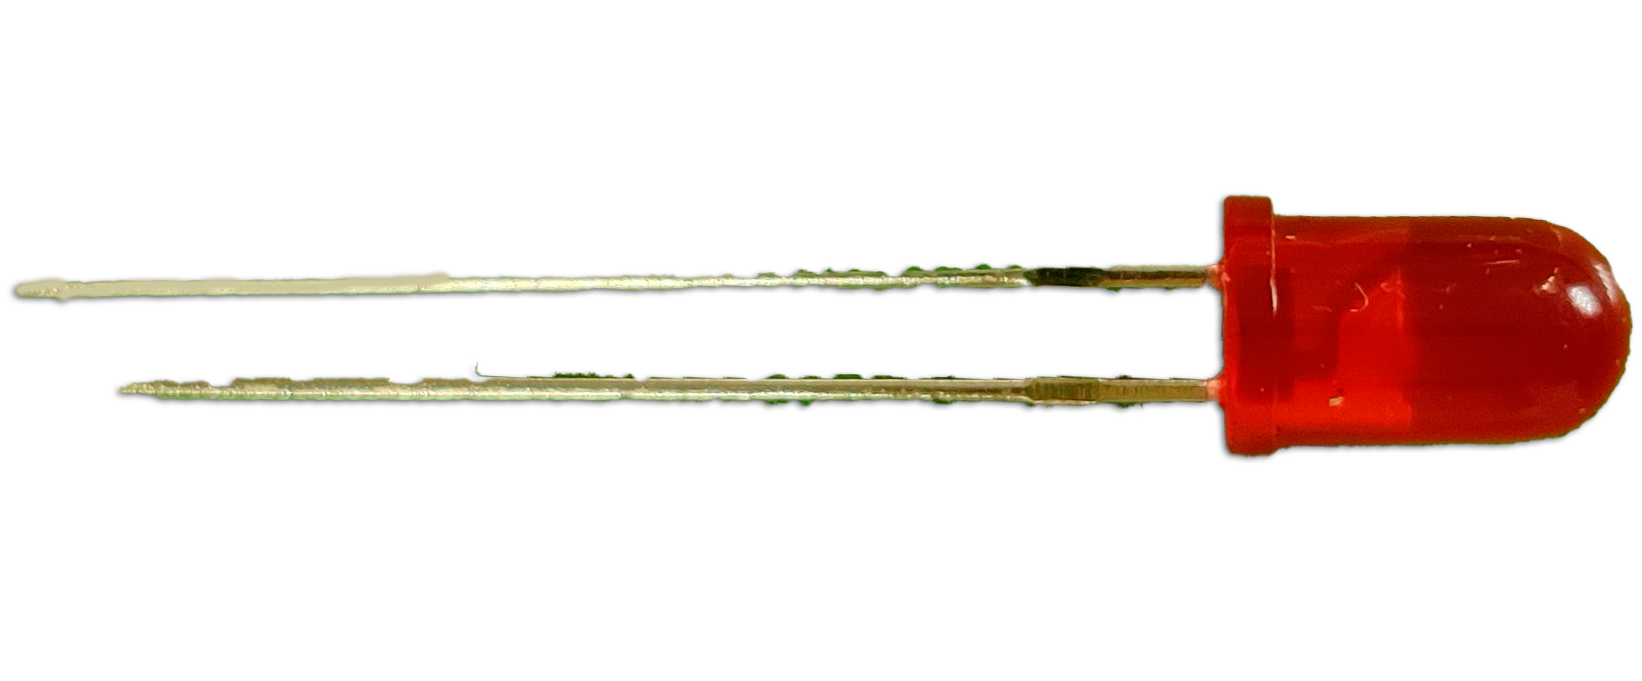
\includegraphics[width=0.95\textwidth]{kuvat/led.png}};
\node[above=0.5] (led) {Anodi (pitkä jalka)};
\node[below=0.5] (led) {Katodi (lyhyt jalka) + tasainen puoli};
\end{tikzpicture}
\end{minipage}

LED, eli valoa säteilevä diodi päästää virtaa läpi vain toiseen suuntaan kuten diodit. Jos anodille kytketään tarpeeksi suuri jännite verrattuna katodiin, virta kulkee ja valo palaa. Jos taas katodilla on suurempi jännite kuin anodilla, virtaa ei kulje ja LED ei pala. Jos anodilla ei ole tarpeeksi suuri jännite verrattuna katodiin, virta ei kulje. Riippuen LEDistä, vaadittu kynnysjännite voi vaihdella ja on tyypillisesti 1,5-4,5 volttia. 
\end{tcolorbox}

\begin{tcolorbox}[title=Jännitelähteen kytkeminen]
Jännitelähde on Arduinossa sisäänrakennettuna. Jotta voimme kytkeä jännitelähteen piiriin, tarvitsemme jännitelähteen molemmat päät: +5V ja maan (GND), kytkemällä vain toinen piiriin emme saa aikaan haluttua vaikutusta.

Arduino levyllä on kolme eri GND-riviä, ja mikä tahansa niistä käy. Kuvassa selvyyden vuoksi ne on numeroitu.

\begin{minipage}{0.3\textwidth}
\begin{tikzpicture}
\ctikzset{american}
\draw (-2,0.5) node[above] {5V} to[short,o-]  (-2,0) to[V,l=$5V$] (-2,-2) to[short,-o] (-2,-2.5) node[below] {GND};
%\node (-2,0.5) {5V};
\end{tikzpicture}
 \end{minipage}
\begin{minipage}{0.7\textwidth}
\begin{tikzpicture}[scale=0.5]
\pic[scale=0.2] at (0,0) {myarduino};
\draw[red,wire] (Ar5V) to[short,*-o] ++(-5,0) node[left,black] {5V};
\draw[black,wire] (ArGND2) to[short,*-o] ++(-5,0) node[left,black] {GND};
\end{tikzpicture}
\end{minipage}
\end{tcolorbox}

\begin{tcolorbox}[title=Painonapin kytkeminen,colback=blue!10,colbacktitle=purple!90]
Arduinon mukana tulevassa painonapissa on neljä pinniä, ja asetetaan keskellä olevan uran ylitse. Jos nappia ei paineta, niin A-E ja F-J rivillä 2 ovat samaa pistettä, mutta eri pistettä kuin rivin 4 (A-E) ja (F-J). Jos nappia painetaan, niin molempien rivien (2 ja 4) kaikki pisteet ovat kiinni toisissaan.


\begin{tikzpicture}[scale=0.5]
\BREADBOARD (0,0) {5};
\draw[thick,fill=hopea] (E2.east) rectangle (F4.west) coordinate[pos=0.5] (Y);
\draw[fill=black] (Y) circle (0.5);
\draw (E2.east) to[short,*-*] (E2);
\draw (E4.east) to[short,*-*] (E4);
\draw (F4.west) to[short,*-*] (F4);
\draw (F2.west) to[short,*-*] (F2);
\end{tikzpicture}
\end{tcolorbox}

\begin{tcolorbox}[title=Lämpötila-anturi,colback=blue!10,colbacktitle=purple!90]
Huomaa, että on merkitystä miten päin lämpötila-anturi kytketään piiriin! 

Jos tasainen sivu on kohti sinua, silloin vasemman puoleisin jalka on käyttöjännite (5V), keskimmäiseltä jalalta (A niin kuin anturi) voidaan lukea tulos ja oikean puoleisin jalka kytketään maahan (GND).

\begin{center}
\begin{tikzpicture}
\node[draw, minimum height=2,color=white,fill=black] (A) at (0,0) {TMP};
\draw[fill=black] (A.north west) to[bend left=70] (A.north east);
\draw[thick] (A.south west)++(0.1,0) --++(0,-0.5) to[short] ++(0,-.5) node[below,left] {5V};
\draw[thick] (A.south) --++(0,-0.5) to[short] ++(0,-.5) node[below] {A};
\draw[thick] (A.south east)++(-0.1,0) --++(0,-0.5) to[short] ++(0,-.5) node[below,right] {GND};
\end{tikzpicture}
\end{center}

Jos kytket anturin väärinpäin, se voi kuumentua. Ole siis tarkkana!
\end{tcolorbox}

\begin{tcolorbox}[title=Valoanturin kytkeminen,colback=blue!10,colbacktitle=purple!90]
Huomaa, että on merkitystä kummin päin valoanturi kytketään koekytkentälevylle! 

Valoanturissa on kaksi jalkaa, joista toinen on pidempi. Valodiodi näyttää kirkkaalta LEDiltä, mutta siitä puuttuu pyöristetty yläosa, eli yläpinta on tasainen (toisin kuin LEDeillä, joilla se on pyöreä). Piirrosmerkissä nuolet tulevat kohti diodia, eli olemme ottamassa valoa sisään (emmekä lähettämässä sitä ulos kuten LEDin kanssa). 

Valoanturin muovi on toiselta puolelta kaareva, ja toiselta siinä on suora leikkaus, lyhyempi jalka on suoran leikkauksen puolella. Lyhyemmän jalan nimi on katodi ja pidemmän jalan anodi.

Piirrosmerkissä:
\begin{center}
\begin{tikzpicture}
%\node at (-1,0) {anodi};
\draw (0,0) node[left,text width=1.5cm] {anodi\\ pitkä jalka} to[photodiode,o-o] (2,0) node[right,text width=2cm] {katodi\\lyhyt jalka};
\end{tikzpicture}
\end{center}

Valodiodi kytketään myös aina vastuksen kanssa sarjaan, nyt käytössä on 10k$\Omega$ vastus. 
\end{tcolorbox}

\begin{tcolorbox}[title=Potentiometrin kytkeminen,colback=blue!10,colbacktitle=purple!90]
Potentiometri on säädettävä vastus, jossa on kolme jalkaa, kaksi toisella puolella ja yksi toisella. Se kytketään uran ylitse, niin että kaksi jaloista ovat toisella puolella ja yksi toisella puolella. Potentiometrin mukana tulee valkoinen säätönuppi, jolla vastuksen arvoa voidaan säädellä pyörittämällä nuppia. 

\begin{minipage}{0.8\textwidth}
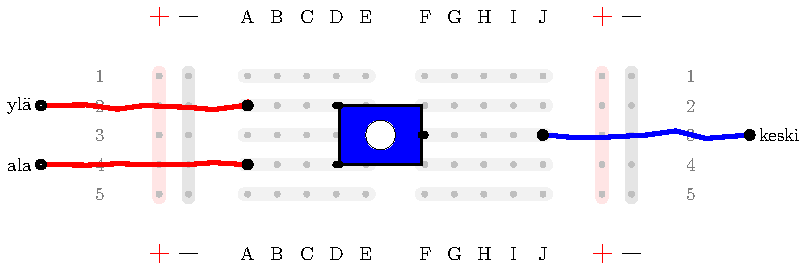
\includegraphics[width=\textwidth]{kuvat/kuva17.pdf}
\end{minipage}%
\begin{minipage}{0.2\textwidth}
Piirrustusmerkki:

\begin{circuitikz} 
\draw (0,0) node[left] {ylä} to[american potentiometer,n=mypot] ++(0,-2) node[right] {ala} (mypot.wiper) to[short] ++(1,0) node[above] {keski};
\end{circuitikz}
\end{minipage}

Mitattaessa vastuksen arvoa välillä ylä-ala, vastuksen arvo pysyy vakiona. Jos taas käytetään vastusta välillä ylä-keski tai keski-ala, vastuksen arvoa voidaan muuttaa pyörittämällä säätönuppia.
\end{tcolorbox}

\begin{tcolorbox}[title=Kaltevuusanturin kytkeminen,colback=blue!10,colbacktitle=purple!90]
Kaltevuusanturissa on neljä jalkaa, ja se vaatii kaksi riviä koekytkentälevystä. Kaltevuusanturi näyttää suorakulmaiselta laatikolta, jonka lähes neliönmuotoisella päällä lukee "UP" ja on nuoli ylös. Tämä rivi, jolla nuoli on, kytketään käyttöjänniteeseen ja toinen rivi kytketään vastuksen kautta maahan. Mittaustulos voidaan lukea samalta riviltä mille vastus on kytketty.  


\begin{tikzpicture}[scale=0.5]
\BREADBOARD (0,0) {5};
\draw[thick,fill=black] (D3.east) rectangle (E4.west) node[pos=0.5,color=white] {UP};
\draw (D3.east) to[short,*-*] (D3);
\draw (D4.east) to[short,*-*] (D4);
\draw (E3.west) to[short,*-*] (E3);
\draw (E4.west) to[short,*-*] (E4);

\draw[wire,red] (A3) to[short,*-o] ++(-7,0) node[left,black] {Käyttöjännite};
\draw[wire,blue] (A4) to[short,*-o] ++(-7,0) node[left,black] {Mittaus};

\end{tikzpicture}
\end{tcolorbox}

\begin{tcolorbox}[title=LCD-näyttö,colback=blue!10,colbacktitle=purple!90]
Tämä on tarkemmin esitelty kappaleessa \ref{sec:lcd} ja tarkemmin kuvassa sivulla \pageref{fig:lcd}. Tällöin LCD-näyttöä ohjataan seuraavilla komennoilla.

\begin{lstlisting}[numbers=none]
#include <LiquidCrystal.h> // Lisataan kirjasto 
LiquidCrystal lcd(13,11,5,4,3,2); // Digital Pinnit joissa kiinni

void setup() {
  lcd.begin(16,2); // Kaynnistetaan naytto
  lcd.print("Tervetuloa"); // Kirjoitetaan ekalle riville
}

void loop() {
  lcd.setCursor(0,1); // Siirrytaan toiselle riville
  lcd.print("Nimi"); // Kirjoita oma nimesi tahan
}
\end{lstlisting}


\end{tcolorbox}